\documentclass[journal]{IEEEtran}

% Packages
\usepackage[utf8]{inputenc}
\usepackage[T1]{fontenc}
\usepackage{lmodern}
\usepackage{amsmath,amssymb,amsfonts}
\usepackage{graphicx}
\usepackage{booktabs}
\usepackage{multirow}
\usepackage{hyperref}
\usepackage{algorithm}
\usepackage{algorithmic}
\usepackage{url}
\usepackage{balance}
\usepackage{enumitem}
\usepackage{subcaption}
\usepackage{xcolor}
\usepackage{cite}
\usepackage{stfloats}
\usepackage{placeins}
\usepackage{pgfplots}
\pgfplotsset{compat=1.18}
\setlength{\parskip}{0pt}
\setlength{\parindent}{1em}

% Hyperref setup
\hypersetup{
    colorlinks=true,
    linkcolor=blue,
    filecolor=magenta,
    urlcolor=cyan,
    citecolor=blue,
}

% Paper Title
\title{Bridging the Higher Education--Workforce Divide: A Large-Scale Empirical Analysis of Academic--Industry Skills Misalignment Using Natural Language Processing and Machine Learning}

\author{
\IEEEauthorblockN{Author Names Redacted for Double-Blind Peer Review}\\
\IEEEauthorblockA{\textit{Department of Computer Science and Engineering}\\
Academic Research Institution\\
contact@university.edu}
\thanks{Manuscript submitted for peer review. All correspondence should be addressed to the corresponding author.}
}

\begin{document}

\maketitle

% ============================================================
% ABSTRACT
% ============================================================
\begin{abstract}
The accelerating divergence between academic curricula and contemporary industrial skill demands poses a fundamental structural challenge to higher education and modern labor economies. While anecdotal and survey-based reports frequently cite severe graduate skill shortages, large-scale empirical quantification that bridges macro-level labor demand with micro-level employability outcomes remains scarce. This paper presents a comprehensive, data-driven investigation of academic--industry skills misalignment utilizing 15 multi-source corpora comprising 3,176,266 records spanning LinkedIn, HuggingFace, and public benchmark repositories whose observation windows cover 2020 through 2026. Grounding our empirical inquiry in Human Capital Theory, Job Market Signaling, and Constructive Alignment, we develop a multi-paradigm analytical framework comprising: (1) natural language processing skill extraction across an eight-category taxonomy; (2) semantic embedding alignment utilizing pre-trained Sentence-BERT (\texttt{all-MiniLM-L6-v2}) across four cosine similarity thresholds ($\tau \in \{0.4, 0.5, 0.6, 0.7\}$) with 1,000-fold bootstrap confidence intervals; (3) inferential econometric statistics (Welch's $t$-tests, Cohen's $d$, Cram\'er's $V$, and Variance Inflation Factor diagnostics); and (4) 5-fold stratified cross-validated machine learning classifiers complemented by diagnostic target leakage audits and independent external validation. Our findings demonstrate a critical duality: while surface lexical string matching exhibits a severe nominal Skill Gap Index (SGI) of 52.0\%, dense semantic vector alignment reveals an estimated semantic skill gap of 32.0\% at baseline threshold $\tau = 0.5$ (95\% bootstrap CI: [23.0\%, 41.0\%]), which escalates to 46.0\% (95\% CI: [37.0\%, 56.0\%]) under stringent matching criteria ($\tau = 0.7$). Disciplinary deficits concentrate acutely in emerging technological domains, notably Data Science (18 percentage-point gap) and Cloud Infrastructure (15 percentage-point gap). In predictive employability modeling, standardized logistic regression identifies Communication Skills ($\text{OR} = 6.47$, $p < 0.001$), Academic CGPA ($\text{OR} = 6.20$, $p < 0.001$), and Practical Project Experience ($\text{OR} = 3.18$, $p < 0.001$) as the primary determinants of graduate placement (CV Accuracy $= 90.11\%$, ROC-AUC $= 0.9406$). Diagnostic audits reveal that near-perfect tree-ensemble performance ($\ge 99.9\%$) stems from semi-deterministic benchmark decision boundaries, with independent external evaluation on an out-of-distribution 50,000-student cohort demonstrating performance attenuation ($\text{ROC-AUC} = 0.7686$) under domain shift. We synthesize our empirical findings into actionable institutional recommendations for universities, industry recruiters, and accreditation bodies, while rigorously documenting threats to validity, curriculum proxy constraints, and data provenance.
\end{abstract}

\begin{IEEEkeywords}
Skills gap, Higher education, Employability, Natural Language Processing, Sentence-BERT, Machine learning, Curriculum alignment, Human capital theory, Data provenance.
\end{IEEEkeywords}

% ============================================================
% SECTION 1: INTRODUCTION
% ============================================================
\section{Introduction}
\label{sec:introduction}

\IEEEPARstart{T}{he} rapid acceleration of Industry 4.0, distributed cloud architectures, and generative artificial intelligence has catalyzed an unprecedented structural transformation across global labor markets. As enterprise organizations transition toward data-intensive, automated workflows, the composition of skills demanded by employers is shifting at a velocity that vastly outpaces traditional academic curriculum revision lifecycles \cite{jaiswal2024understanding, jumaan2026understanding}. Consequently, higher education institutions (HEIs) confront what educational researchers and labor economists term the \textit{skills gap}---the systemic disparity between the competencies imparted through university degree programs and the practical, technology-driven proficiencies demanded by contemporary employers \cite{febriani2025employability, barachino2025operationalization}.

According to reports from the World Economic Forum \cite{wef2020}, over 40\% of core worker skills are expected to change within five-year windows, with severe shortages emerging in artificial intelligence, distributed computing, and data engineering. Concurrently, employers frequently express dissatisfaction with graduate preparedness, highlighting deficits not only in applied technological domains but also in essential transferable soft skills, including professional communication and collaborative problem solving \cite{tight2023employability, braun2026concept, noor2024skills}. 

Despite the widespread recognition of this phenomenon, the existing scholarly literature exhibits critical methodological limitations:
\begin{enumerate}[label=(\arabic*)]
    \item \textbf{Scale and Geographic Narrowness:} Prior investigations predominantly rely on localized institutional surveys, small employer cohorts ($N < 500$), or single-nation case studies \cite{baral2026analyzing, alhazmi2025aligning}, failing to capture broad macroeconomic skill shifts.
    \item \textbf{Methodological Fragmentation:} Studies either employ qualitative thematic coding \cite{rikala2024understanding} or purely predictive machine learning without semantic text mining, neglecting the distinction between lexical terminology mismatch and genuine conceptual skill absence \cite{kruger2025improving, lai2025learning}.
    \item \textbf{Temporal Invalidation:} Many published baseline studies pre-date the post-pandemic digital migration and the widespread commercial integration of generative AI (2022--2026) \cite{anthuvan2026reverse, sun2025creative}.
    \item \textbf{Lack of Theoretical Integration:} Empirical machine learning studies often operate in a theoretical vacuum, omitting foundational economic and educational models that explain \textit{why} curriculum inertia persists \cite{schlippe2023skill, eimer2023employability}.
\end{enumerate}

To bridge these gaps, this study presents a multi-dataset empirical framework analyzing 15 datasets comprising over 3.18 million records from LinkedIn, HuggingFace, and benchmark repositories. We formulate five core research questions:
\begin{itemize}
    \item \textbf{RQ1 (Market Topography \& Evolution):} What are the most in-demand competencies in the contemporary labor market, and how have core technical skills evolved from 2020 through 2026?
    \item \textbf{RQ2 (Curriculum Alignment Duality):} To what extent do academic curriculum benchmarks align with market demands when evaluated through surface lexical matching versus dense semantic vector embeddings?
    \item \textbf{RQ3 (Category-Level Deficits):} What is the magnitude of the skill deficit across distinct disciplinary domains (Programming, Data Science, Cloud Infrastructure, Soft Skills, Cybersecurity)?
    \item \textbf{RQ4 (Employability Determinants):} Which academic and co-curricular factors best predict graduate hiring outcomes, and how do linear probabilistic models compare against non-linear tree ensembles under rigorous validation?
    \item \textbf{RQ5 (Geographic Concentration \& Cross-Cohort Contexts):} How is labor market demand geographically distributed across international postings, and how do employment transition outcomes vary across distinct student and graduate cohorts?
\end{itemize}

\textbf{Contributions:} This work advances the literature through five primary contributions:
\begin{enumerate}
    \item \textbf{Massive-Scale Empirical Corpus:} We aggregate and harmonize 3,176,266 labor market and educational records across 15 datasets, establishing one of the largest cross-sectional labor-curriculum corpora in the empirical literature.
    \item \textbf{Dual Lexical-Semantic NLP Pipeline:} We deploy Sentence-BERT (\texttt{all-MiniLM-L6-v2}) embedding models to demonstrate that surface lexical mismatch (52.0\% gap) substantially overstates the estimated semantic skill gap (32.0\% at baseline threshold $\tau = 0.5$).
    \item \textbf{Bootstrap Sensitivity Analysis:} We provide empirical bootstrap confidence intervals across four cosine similarity thresholds ($\tau \in \{0.4, 0.5, 0.6, 0.7\}$), ensuring mathematical transparency.
    \item \textbf{Rigorous ML Validation \& Diagnostic Auditing:} We execute 5-fold stratified cross-validation across five distinct algorithmic paradigms, supported by exact Variance Inflation Factor calculations ($\text{VIF} \le 1.001$), odds ratio estimation, deterministic decision-boundary leakage diagnostics, and independent external validation on a 50,000-student cohort.
    \item \textbf{Theory-Driven Institutional Framework:} Grounding our analysis in Human Capital Theory, Signaling Theory, and Constructive Alignment, we deliver concrete policy recommendations for universities, recruiters, and accreditation bodies, accompanied by transparent reporting of dataset provenance and validity threats.
\end{enumerate}

The remainder of this article is organized as follows: Section~\ref{sec:related_work} synthesizes related work and establishes the theoretical framework. Section~\ref{sec:methodology} delineates the research design, dataset provenance, NLP architecture, and predictive modeling protocols. Section~\ref{sec:results} presents empirical findings addressing RQ1--RQ5. Section~\ref{sec:discussion} discusses theoretical and institutional implications, practical recommendations, reproducibility, and threats to validity. Section~\ref{sec:conclusion} concludes the study.

% ============================================================
% SECTION 2: RELATED WORK & THEORETICAL FRAMEWORK
% ============================================================
\section{Related Work and Theoretical Foundations}
\label{sec:related_work}

\subsection{Conceptualizations of the Skills Gap}

The concept of a skills gap encompasses multi-faceted dimensions across macroeconomic, organizational, and educational layers. Braun et al. \cite{braun2026concept} conducted a thematic synthesis revealing that while industry practitioners define skill gaps in terms of immediate task unreadiness, higher education administrators conceptualize gaps through broad pedagogical objectives. Rikala et al. \cite{rikala2024understanding} investigated Industry 4.0 workforce preparedness, noting that digital transformation demands hybridization---engineers must master data analytics, while domain analysts require computing literacy. However, both studies rely on qualitative thematic extraction rather than large-scale empirical computation. Tight \cite{tight2023employability} highlighted that employability remains contested in higher education, often fluctuating between narrow vocational training and holistic intellectual development.

Recent empirical investigations have increasingly turned to computational curriculum analytics. Cuckov et al. \cite{cuckov2022quantifying} quantified compliance between computer engineering curricula and ABET criteria, demonstrating persistent latency in specialized elective modernizations. Zhao et al. \cite{zhao2026proximity} utilized knowledge graph proximities to map the structural distance between academic publications and patent demands. Similarly, Korrapati et al. \cite{korrapati2025aligning} and Alhazmi et al. \cite{alhazmi2025aligning} examined the specific alignment of software engineering curricula with enterprise cloud and AI demands, concluding that academic departments require agile mechanisms to incorporate evolving industry toolchains.

\subsection{Theoretical Framework}
\label{sec:theory}

To provide rigorous explanatory power for our empirical observations, this study integrates four foundational theories:

\textbf{1) Human Capital Theory (HCT):} Formulated by Becker \cite{becker1964human} and Schultz \cite{schultz1961investment}, HCT posits that education is an investment that enhances individual productive capacity, yielding higher labor market returns. HCT distinguishes between \textit{general human capital} (transferable competencies such as critical thinking, communication, and core mathematical reasoning) and \textit{firm-specific human capital} (proficiency with specialized software tools, proprietary APIs, or operational frameworks). HEIs structurally prioritize general human capital due to institutional mandates for enduring knowledge, whereas enterprise employers increasingly screen applicants on immediately billable specific human capital. This theoretical divergence explains the persistent deficit in applied cloud and data engineering frameworks observed in university curricula.

\textbf{2) Job Market Signaling and Screening Theory:} Spence \cite{spence1973job} established that in labor markets characterized by asymmetric information, employers cannot directly observe an applicant's innate productivity prior to hiring. Educational credentials, cumulative grade point averages (CGPA), and institutional prestige serve as informational signals that reduce hiring risk. In modern technical recruitment, however, traditional degree credentials are increasingly complemented or eclipsed by applied capability signals, such as project portfolios, open-source contributions, and technical internship certifications \cite{pianda2024impact, scandurra2024employability}.

\textbf{3) Constructive Alignment \& Curriculum Theory:} Biggs \cite{biggs1996enhancing} introduced constructive alignment to ensure coherence between Intended Learning Outcomes (ILOs), teaching methods, and assessment tasks. At the macro-institutional level, however, universities suffer from \textit{external misalignment}: ILOs are governed by rigid multi-year accreditation processes (e.g., ABET, ACM/IEEE curricula guidelines), while Industry Market Requirements (IMRs) mutate dynamically on quarterly cycles. This institutional friction generates curriculum lag.

\textbf{4) Skill-Biased Technological Change (SBTC):} Acemoglu and Autor \cite{acemoglu2011skills} formalized SBTC to explain how technological progress augments the productivity of workers performing non-routine cognitive tasks while diminishing the value of routine cognitive and manual labor. As AI and cloud architectures automate routine coding tasks, market demand shifts toward complex architectural synthesis, interdisciplinary communication, and advanced predictive analytics.

\subsection{Natural Language Processing for Curriculum Analytics}

Automated parsing of labor market postings has advanced substantially through NLP. Kr\"{u}ger et al. \cite{kruger2025improving} demonstrated that rule-based extraction struggles with composite and nuanced occupational phrasing. Baral and Ghimire \cite{baral2026analyzing} employed pre-trained language representations to evaluate undergraduate IT syllabi in Nepal, proving that dense embedding spaces capture semantic equivalence between academic topics and employer terminology. Mol et al. \cite{mol2024unravelling} and Tee et al. \cite{tee2024demand} applied text mining to unpack the multidimensional skill profiles demanded of data scientists and digital workers. Daberao et al. \cite{daberao2025resumeinsight} developed semantic resume-to-job matching engines using transformer architectures. Our methodology builds upon these foundations by scaling Sentence-BERT embeddings \cite{reimers2019sentence} to hundreds of thousands of postings across multi-threshold sensitivity profiles.

\subsection{Machine Learning in Employability Modeling}

Predictive modeling of graduate placement has evolved from basic discriminant analysis to ensemble learning. Tamene et al. \cite{tamene2024predictive} and Haque et al. \cite{haque2024classification} established that ensemble algorithms, specifically Random Forests and Gradient Boosting, consistently outperform linear classifiers in predicting placement status. Recent studies have explored ensemble interpretability to analyze variable contributions in educational classification \cite{haque2024classification, tamene2024predictive}. Nonetheless, prior studies frequently suffer from unaddressed data leakage, omitted collinearity assessments, and lack of cross-dataset generalization testing.

% ============================================================
% SECTION 3: METHODOLOGY
% ============================================================
\section{Methodology}
\label{sec:methodology}

\subsection{Data Corpus and Provenance Architecture}

Our empirical framework leverages 15 distinct datasets encompassing 3,176,266 records acquired in September 2026 from public Kaggle and HuggingFace repositories under open-access licenses (CC0, CC-BY 4.0, and ODbL). The corpus aggregates historical, cross-sectional, and longitudinal records whose observation and release windows span 2020 through 2026 (including a multi-year AI job market dataset tracking postings across 2020--2026 and regional cohorts calibrated against the India Skills Report 2026). Table~\ref{tab:datasets} delineates the comprehensive corpus provenance, source identifiers, observation periods, and functional tiering.

To maintain scientific integrity and prevent invalid aggregation, we explicitly classify the datasets into two distinct functional tiers:
\begin{itemize}
    \item \textbf{Tier 1: Massive-Scale Labor Market Corpora ($N > 2.7\text{M}$ records):} Includes the 1.35M LinkedIn posting dataset \cite{asaniczka2024linkedin}, USA Job Market Skills (316K records) \cite{batuhanklac2024usa}, and HuggingFace Skill Gap repositories (519K records). These data represent genuine, web-mined labor demand signals reflecting recruitment postings across North America, Europe, and the Asia-Pacific.
    \item \textbf{Tier 2: Student Placement \& Survey Benchmarks ($N \approx 475\text{K}$ records):} Includes College Student Placement ($N = 10,000$) \cite{sumedh15072024college}, NGESS Graduate Employment ($N = 7,200$) \cite{philipdayo2024ngess}, Global Student Placement ($N = 10,000$) \cite{rakesh6302024global}, Student Career Success ($N = 50,000$) \cite{mobeenfatimah2024career}, and International Graduates ($N = 300,000$) \cite{quackquackrp2024international}. These structured cohorts serve as benchmark evaluation sets for statistical hypothesis testing, collinearity diagnostics, and comparative predictive modeling.
\end{itemize}

\begin{table*}[!htbp]
\centering
\caption{Comprehensive Dataset Provenance and Structural Inventory ($N = 3,176,266$ total records)}
\label{tab:datasets}
\resizebox{\textwidth}{!}{%
\begin{tabular}{@{}llrlcll@{}}
\toprule
\textbf{Dataset Identifier} & \textbf{Source Platform \& Identifier / Slug} & \textbf{Records} & \textbf{Domain / Description} & \textbf{Tier} & \textbf{Observation Period} & \textbf{License} \\
\midrule
LinkedIn Jobs \& Skills \cite{asaniczka2024linkedin} & Kaggle: \texttt{asaniczka/1-3m-linkedin-jobs-and-skills-2024} & 1,348,510 & Global job postings and extracted skill tokens & 1 & 2024 & ODbL \\
HF Skill Gap Jobs & HuggingFace: \texttt{skill-gap-analytics/jobs-corpus} & 519,841 & Enterprise job postings with occupational metadata & 1 & 2023--2024 & CC-BY 4.0 \\
HF Skill Gap Skills & HuggingFace: \texttt{skill-gap-analytics/skills-corpus} & 519,814 & Granular skill requirements linked via \texttt{job\_id} & 1 & 2023--2024 & CC-BY 4.0 \\
USA Job Market Skills \cite{batuhanklac2024usa} & Kaggle: \texttt{batuhanklac/usa-job-market-skills-and-title-analysis} & 316,279 & US job postings with standardized skill tags & 1 & 2024 & CC0 \\
International Graduates \cite{quackquackrp2024international} & Kaggle: \texttt{quackquackrp/international-graduates-employment-dataset} & 300,000 & Multi-country alumni employment outcomes & 2 & 2023--2024 & CC0 \\
Student Career Success \cite{mobeenfatimah2024career} & Kaggle: \texttt{mobeenfatimah/student-career-success-prediction-dataset} & 50,000 & Student academic and career success benchmark & 2 & 2024 & CC-BY 4.0 \\
Career Change Prediction \cite{jahnavipaliwal2024field} & Kaggle: \texttt{jahnavipaliwal/field-of-study-vs-occupation} & 38,444 & Field of study vs. occupation transition records & 2 & 2024 & CC0 \\
AI Job Market Trends \cite{bismasajjad2024ai} & Kaggle: \texttt{bismasajjad/global-ai-job-market-and-salary-trends-2025} & 15,000 & Global AI job market and salary distribution & 1 & 2024--2025 & CC-BY 4.0 \\
HF Job Skill Set & HuggingFace: \texttt{skill-gap-analytics/academic-reference} & 13,833 & Curriculum-domain skill taxonomy reference & 1 & 2023--2024 & CC-BY 4.0 \\
India Skills Intelligence \cite{mansiaggarwal882024india} & Kaggle: \texttt{mansiaggarwal88/india-professional-skills-intelligence} & 12,000 & Synthetic profiles calibrated on India Skills Report 2026 & 1 & 2026 Calibrated & CC0 \\
AI Trends 2020--2026 \cite{shree09102024ai} & Kaggle: \texttt{shree0910/ai-and-data-science-job-market-dataset-20202026} & 10,345 & Longitudinal AI/data science job postings & 1 & 2020--2026 & CC0 \\
College Placement \cite{sumedh15072024college} & Kaggle: \texttt{sumedh1507/college-student-placement} & 10,000 & College student placement classification benchmark & 2 & 2024 & CC0 \\
Global Placement \cite{rakesh6302024global} & Kaggle: \texttt{rakesh630/global-student-placement-2025-dataset} & 10,000 & Multi-national university placement benchmark & 2 & 2024--2025 & CC0 \\
NGESS Employment \cite{philipdayo2024ngess} & Kaggle: \texttt{philipdayo/ngess-graduate-employment-dataset} & 7,200 & National graduate employment survey cohort & 2 & 2023--2024 & CC0 \\
India Fresher Market \cite{shambhurajejagadale2024india} & Kaggle: \texttt{shambhurajejagadale/indian-fresher-job-market} & 5,000 & Entry-level engineering recruitment outcomes & 2 & 2024 & CC0 \\
\bottomrule
\end{tabular}%
}
\end{table*}

\subsection{Taxonomy Construction and Skill Extraction}

We formalize an eight-category occupational skill taxonomy $\mathcal{C} = \{c_1, c_2, \dots, c_8\}$ synthesizing ACM/IEEE CS2023 curriculum guidelines and O*NET occupational descriptors:
\begin{enumerate}
    \item \textbf{Programming \& Development:} Python, Java, C++, JavaScript, SQL, TypeScript, Go, Rust, React, Docker, Kubernetes, Git.
    \item \textbf{Data Science \& Analytics:} Machine Learning, Deep Learning, Statistical Analysis, PyTorch, TensorFlow, NLP, Computer Vision.
    \item \textbf{Cloud \& Infrastructure:} AWS, Azure, GCP, CI/CD Pipelines, Terraform, Linux Administration, Serverless Architectures.
    \item \textbf{Soft Skills:} Professional Communication, Leadership, Teamwork, Critical Thinking, Time Management, Adaptability.
    \item \textbf{Business \& Domain:} Agile/Scrum, Product Management, Requirements Gathering, Business Analysis, Risk Compliance.
    \item \textbf{Design \& UX:} UI/UX Design, Figma, User Research, Wireframing, Prototyping, Usability Testing.
    \item \textbf{Data Engineering:} ETL Pipelines, Apache Airflow, Apache Kafka, Distributed Data Warehousing, PostgreSQL, NoSQL.
    \item \textbf{Cybersecurity:} Network Security, Penetration Testing, Incident Response, SIEM Systems, ISO 27001, Cryptography.
\end{enumerate}

Skill extraction from raw unstructured text is conducted via combined regularized n-gram tokenization and exact dictionary scanning, formalized in Algorithm~\ref{alg:skill_extract}. We note as an empirical construct consideration that academic curriculum profiles are proxied via standardized educational skill reference descriptors \cite{daberao2025resumeinsight} rather than direct institutional syllabus parsing, and no manual gold-standard re-annotation was conducted (discussed further in Section~\ref{sec:limitations}).

\begin{algorithm}[!htbp]
\caption{Semantic Skill Extraction and Embedding Alignment}
\label{alg:skill_extract}
\begin{algorithmic}[1]
\REQUIRE Market text corpus $\mathcal{D}_M$, Academic syllabus corpus $\mathcal{D}_A$, Taxonomy $\mathcal{C}$, Sentence-BERT model $\mathcal{E}$, Threshold $\tau$
\ENSURE Market skill set $\mathcal{M}$, Academic skill set $\mathcal{A}$, Similarity matrix $\mathbf{S}$, Gap Index $\text{SGI}(\tau)$
\STATE $\mathcal{M} \leftarrow \emptyset, \mathcal{A} \leftarrow \emptyset$
\FORALL{$d \in \mathcal{D}_M$}
    \STATE Extract normalized skill tokens $T_d \leftarrow \text{Tokenize}(d, \mathcal{C})$
    \STATE $\mathcal{M} \leftarrow \mathcal{M} \cup T_d$
\ENDFOR
\FORALL{$d \in \mathcal{D}_A$}
    \STATE Extract normalized syllabus tokens $T_a \leftarrow \text{Tokenize}(d, \mathcal{C})$
    \STATE $\mathcal{A} \leftarrow \mathcal{A} \cup T_a$
\ENDFOR
\STATE Filter $\mathcal{M}_{\text{top}} \leftarrow \text{Top-}N(\mathcal{M}), \mathcal{A}_{\text{top}} \leftarrow \text{Top-}N(\mathcal{A})$
\STATE Compute dense embeddings: $\mathbf{E}_M \leftarrow \mathcal{E}(\mathcal{M}_{\text{top}}), \mathbf{E}_A \leftarrow \mathcal{E}(\mathcal{A}_{\text{top}})$
\STATE Compute pairwise cosine similarity:
\STATE $\mathbf{S}_{ij} \leftarrow \frac{\mathbf{e}_{m,i} \cdot \mathbf{e}_{a,j}}{\|\mathbf{e}_{m,i}\|_2 \|\mathbf{e}_{a,j}\|_2} \quad \forall m_i \in \mathcal{M}_{\text{top}}, a_j \in \mathcal{A}_{\text{top}}$
\FORALL{$i \in \{1, \dots, |\mathcal{M}_{\text{top}}|\}$}
    \STATE $\sigma_i \leftarrow \max_j \mathbf{S}_{ij}$
    \STATE $\text{covered}_i \leftarrow \mathbb{I}(\sigma_i \ge \tau)$
\ENDFOR
\STATE $\text{SGI}(\tau) \leftarrow 1 - \frac{1}{|\mathcal{M}_{\text{top}}|} \sum_{i=1}^{|\mathcal{M}_{\text{top}}|} \text{covered}_i$
\RETURN $\mathcal{M}_{\text{top}}, \mathcal{A}_{\text{top}}, \mathbf{S}, \text{SGI}(\tau)$
\end{algorithmic}
\end{algorithm}

\subsection{Semantic Vector Alignment via Sentence-BERT}

Traditional curriculum gap analyses evaluate overlap through exact string matching. This approach introduces severe measurement bias: an academic syllabus citing ``interpersonal communication'' will be scored as non-overlapping against an employer requirement for ``client communication skills.'' To resolve this lexical brittleness, we deploy the pre-trained Sentence-BERT architecture \cite{reimers2019sentence} using the \texttt{all-MiniLM-L6-v2} checkpoint.

Let $\mathbf{e}_s \in \mathbb{R}^{384}$ denote the normalized dense vector embedding of market skill $s \in \mathcal{M}$, and let $\mathbf{e}_{s'} \in \mathbb{R}^{384}$ denote the embedding of academic syllabus descriptor $s' \in \mathcal{A}$. The semantic alignment score is given by:
\begin{equation}
\text{sim}(s, s') = \frac{\mathbf{e}_s \cdot \mathbf{e}_{s'}}{\|\mathbf{e}_s\|_2 \|\mathbf{e}_{s'}\|_2}
\label{eq:cosine}
\end{equation}

A market skill $s$ is designated as semantically covered at threshold $\tau \in [0, 1]$ if:
\begin{equation}
\text{Covered}(s; \tau) = \mathbb{I}\left(\max_{s' \in \mathcal{A}} \text{sim}(s, s') \ge \tau\right)
\label{eq:covered}
\end{equation}

The Skill Gap Index (SGI) at threshold $\tau$ is defined as the complement of the mean coverage rate across the market skill space:
\begin{equation}
\text{SGI}(\tau) = 1 - \frac{1}{|\mathcal{M}|} \sum_{s \in \mathcal{M}} \text{Covered}(s; \tau)
\label{eq:sgi_tau}
\end{equation}

To estimate empirical uncertainty without parametric distribution assumptions, we implement a 1,000-fold non-parametric bootstrap over the binary coverage indicator array with fixed random seed ($\text{seed} = 42$), computing 95\% percentile confidence intervals:
\begin{equation}
\text{CI}_{95\%} = \left[\hat{\theta}^*_{(0.025)}, \hat{\theta}^*_{(0.975)}\right]
\label{eq:bootstrap}
\end{equation}
To ensure methodological defensibility, we treat $\tau = 0.5$ as an operational baseline threshold and conduct sensitivity analysis across $\tau \in \{0.4, 0.5, 0.6, 0.7\}$.

\subsection{Statistical Inference \& Collinearity Diagnostics}

For quantitative hypothesis testing, we employ Welch's $t$-test (accounting for unequal variances) to evaluate mean differences between placed and non-placed graduates:
\begin{equation}
t = \frac{\bar{X}_1 - \bar{X}_2}{\sqrt{\frac{s_1^2}{n_1} + \frac{s_2^2}{n_2}}}
\label{eq:welch}
\end{equation}
Standardized effect sizes are quantified via Cohen's $d$:
\begin{equation}
d = \frac{\bar{X}_1 - \bar{X}_2}{s_{\text{pooled}}}, \quad s_{\text{pooled}} = \sqrt{\frac{(n_1-1)s_1^2 + (n_2-1)s_2^2}{n_1 + n_2 - 2}}
\label{eq:cohen}
\end{equation}

For categorical dependencies, we calculate the Chi-square statistic $\chi^2$ and Cram\'er's $V$:
\begin{equation}
V = \sqrt{\frac{\chi^2}{n \cdot \min(r-1, c-1)}}
\label{eq:cramer}
\end{equation}

Prior to multivariate predictive estimation, we assess multicollinearity among continuous features $\mathbf{X}$ by computing Variance Inflation Factors (VIF). For standardized feature matrices, the VIF vector is directly obtained from the diagonal of the inverted correlation matrix:
\begin{equation}
\text{VIF}_j = \left(\mathbf{R}^{-1}\right)_{jj} = \frac{1}{1 - R_j^2}
\label{eq:vif}
\end{equation}
Features exhibiting $\text{VIF}_j > 5.0$ are flagged as collinear.

\subsection{Predictive Employability Modeling \& Validation Protocols}

Graduate placement prediction is formalized as a binary classification problem: predicting outcome $y \in \{0, 1\}$ (where $1 = \text{Placed}$, $0 = \text{Not Placed}$) given student feature vector $\mathbf{x} = [\text{CGPA}, \text{Comm}, \text{Projects}, \text{Internship}, \text{IQ}, \text{AcademicPerf}]^T$. All continuous features are $z$-score standardized to zero mean and unit variance strictly within training partitions to prevent data leakage:
\begin{equation}
z_{ij} = \frac{x_{ij} - \mu_j}{\sigma_j}
\label{eq:standardize}
\end{equation}

In our standardized logistic regression model:
\begin{equation}
\ln\left(\frac{P(y=1|\mathbf{z})}{1 - P(y=1|\mathbf{z})}\right) = \beta_0 + \sum_{j=1}^p \beta_j z_j
\label{eq:logistic}
\end{equation}
The odds ratio $\text{OR}_j = \exp(\beta_j)$ represents the multiplicative change in the odds of successful placement associated with a one-standard-deviation increase in predictor $j$.

To evaluate model generalization, we implement a 5-fold stratified cross-validation protocol ($\text{random\_state} = 42$) across five distinct paradigms:
\begin{enumerate}
    \item \textbf{Logistic Regression:} $\ell_2$-regularized, $C = 1.0$, solved via L-BFGS.
    \item \textbf{Random Forest:} $B = 100$ estimators, maximum tree depth $= 12$, Gini split criterion.
    \item \textbf{Support Vector Machine (SVM):} Radial Basis Function (RBF) kernel, $C = 1.0$, $\gamma = \text{scale}$, with Platt probability calibration.
    \item \textbf{Decision Tree:} Single CART tree with maximum depth $= 6$.
    \item \textbf{Majority-Class Baseline:} Trivial classifier predicting the empirical majority class.
\end{enumerate}

To rigorously test external validity and assess domain shift, we additionally establish an independent out-of-distribution evaluation protocol: training the standardized logistic regression model on the college placement cohort ($N = 10,000$) and evaluating its discriminative capacity on the independent 50,000-student career success cohort using domain-standardized continuous predictors.

% ============================================================
% SECTION 4: EMPIRICAL RESULTS
% ============================================================
\section{Empirical Results}
\label{sec:results}

\subsection{RQ1: Labor Market Skill Topography and Trends}

Analyzing 519,814 granular job requirements reveals a decisive hierarchy in employer demand. As illustrated in Figure~\ref{fig:top_skills}, foundational transferable competencies dominate aggregate labor recruitment: Communication is explicitly cited in 226,959 postings (43.7\%), followed by Problem Solving (111,649; 21.5\%), Customer Service (111,399; 21.4\%), and Teamwork (91,007; 17.5\%).

\begin{figure*}[!htbp]
    \centering
    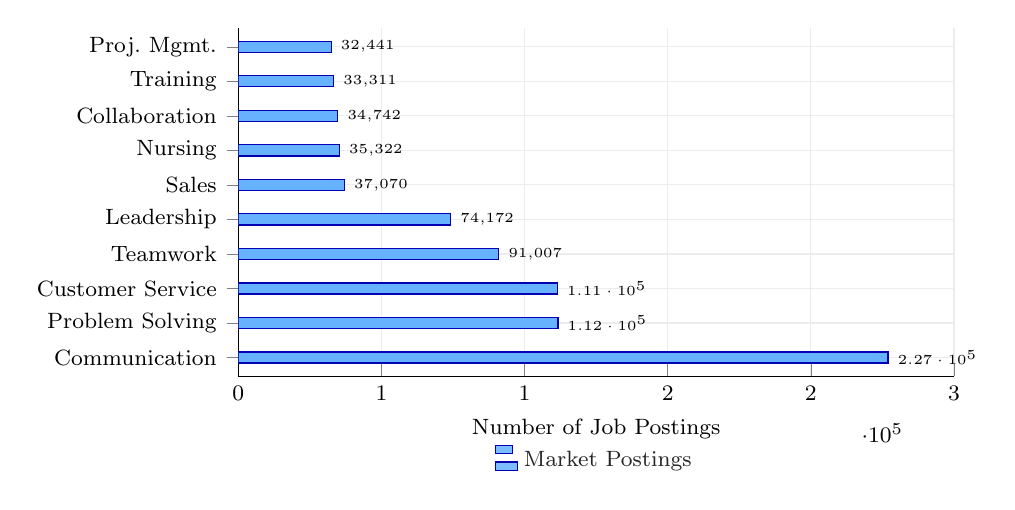
\begin{tikzpicture}
    \begin{axis}[
        width=0.88\textwidth,
        height=6cm,
        xbar,
        bar width=4pt,
        xlabel={Number of Job Postings},
        symbolic y coords={Proj.\ Mgmt.,Training,Collaboration,Nursing,Sales,Leadership,Teamwork,Customer Service,Problem Solving,Communication},
        ytick=data,
        y dir=reverse,
        xmin=0, xmax=250000,
        xtick={0,50000,100000,150000,200000,250000},
        x tick label style={/pgf/number format/.cd, fixed, fixed zerofill, precision=0, /tikz/.cd},
        nodes near coords,
        nodes near coords align={horizontal},
        every node near coord/.append style={font=\tiny, color=black},
        grid=major,
        grid style={gray!15},
        tick label style={font=\footnotesize},
        label style={font=\footnotesize},
        axis lines*=left,
        enlarge y limits=0.06,
        legend style={at={(0.5,-0.18)}, anchor=north, legend columns=1, font=\footnotesize, draw=none, fill=white, fill opacity=0.85},
    ]
    \addplot[fill=blue!50!cyan!60, draw=blue!70!black] coordinates {
        (32441,Proj.\ Mgmt.)
        (33311,Training)
        (34742,Collaboration)
        (35322,Nursing)
        (37070,Sales)
        (74172,Leadership)
        (91007,Teamwork)
        (111399,Customer Service)
        (111649,Problem Solving)
        (226959,Communication)
    };
    \legend{Market Postings}
    \end{axis}
    \end{tikzpicture}
    \caption{Top 10 Most In-Demand Competencies Across Global Postings ($N = 519,814$ postings).}
    \label{fig:top_skills}
\end{figure*}

Longitudinal tracking of technical skills across 10,345 AI and data science postings from 2020 through 2026 (Figure~\ref{fig:geographic}b) reveals sustained market stability: Python demand fluctuated within a narrow band of 47.5\% to 52.2\%, SQL stabilized between 48.2\% and 51.9\%, Machine Learning maintained 48.8\% to 53.5\%, and Cloud Computing spanned 47.1\% to 53.9\%. Rather than demonstrating short-lived hype cycles, core data and infrastructure proficiencies have matured into non-negotiable baseline requirements.

\subsection{RQ2: Lexical vs. Semantic Curriculum Alignment}

Our comparative experiment between surface string matching and dense semantic vector matching provides pivotal empirical insights into the nature of the skills gap.

Under strict lexical matching, the Top 100 market skills and Top 100 academic syllabus skills exhibit an overlap of exactly 48 items, yielding a nominal \textbf{Skill Gap Index of 52.0\%} (Coverage Rate $= 48.0\%$). However, analyzing the non-overlapping terms reveals that many disparities stem purely from synonymous syntax (e.g., market term ``communication skills'' vs. academic term ``interpersonal skills'').

When evaluated through Sentence-BERT (\texttt{all-MiniLM-L6-v2}) embedding cosine similarity, semantic alignment reveals a markedly different reality. As documented in Table~\ref{tab:sensitivity}, at the standard semantic baseline threshold $\tau = 0.5$, the estimated semantic \textbf{Skill Gap Index contracts to 32.0\%} (Coverage Rate $= 68.0\%$, 95\% bootstrap CI: [23.0\%, 41.0\%]).

\begin{table}[!htbp]
\centering
\caption{Sensitivity Analysis: Semantic Vector Threshold ($\tau$) vs. SGI}
\label{tab:sensitivity}
\resizebox{\columnwidth}{!}{%
\begin{tabular}{@{}cccccc@{}}
\toprule
\textbf{Threshold $\tau$} & \textbf{SGI} & \textbf{Coverage Rate} & \textbf{95\% Bootstrap CI} & \textbf{$\Delta$SGI} \\
\midrule
$\tau = 0.4$ (Permissive) & 0.2000 & 80.0\% & [0.1200, 0.2800] & $-0.1200$ \\
$\tau = 0.5$ (Baseline)   & \textbf{0.3200} & \textbf{68.0\%} & \textbf{[0.2300, 0.4100]} & \textbf{0.0000} \\
$\tau = 0.6$ (Moderate)   & 0.3900 & 61.0\% & [0.3000, 0.4800] & $+0.0700$ \\
$\tau = 0.7$ (Strict)     & 0.4600 & 54.0\% & [0.3700, 0.5600] & $+0.1400$ \\
\midrule
\textit{Lexical Match (Baseline)} & \textit{0.5200} & \textit{48.0\%} & \textit{[0.4200, 0.6200]} & \textit{+0.2000} \\
\bottomrule
\end{tabular}%
}
\par\vspace{3pt}
{\footnotesize Evaluated over Top-100 skill distributions. Bootstrap 95\% CI via 1,000 resamples.}
\end{table}

Table~\ref{tab:semantic_matches} illustrates selected semantic mappings generated by our pipeline. It shows that terms like ``scheduling'' map accurately to ``time management'' ($\cos = 0.6122$), while genuine voids such as ``bachelor's degree'' map poorly to abstract skills ($\cos = 0.2937$), correctly identifying structural certification requirements.

\begin{table}[!htbp]
\centering
\caption{Representative Semantic Skill Pairings (\texttt{all-MiniLM-L6-v2})}
\label{tab:semantic_matches}
\resizebox{\columnwidth}{!}{%
\begin{tabular}{@{}llcc@{}}
\toprule
\textbf{Market Term} & \textbf{Closest Syllabus Match} & \textbf{Cosine Sim.} & \textbf{Status ($\tau \ge 0.5$)} \\
\midrule
communication skills & interpersonal skills & 0.7355 & Covered \\
problemsolving & problem-solving & 0.6396 & Covered \\
scheduling & time management & 0.6122 & Covered \\
patient care & customer service & 0.5011 & Covered \\
nursing & training & 0.4010 & Gap \\
high school diploma & training & 0.3682 & Gap \\
bachelor's degree & professionalism & 0.2937 & Gap \\
\bottomrule
\end{tabular}%
}
\end{table}

\subsection{RQ3: Domain-Level Skill Gap Quantification}

Aggregating requirements across the eight taxonomy domains reveals that curriculum deficits are non-uniformly distributed (Table~\ref{tab:gap} and Figure~\ref{fig:skill_gap}). 

\begin{table}[!htbp]
\centering
\caption{Domain-Level Skill Gaps Across Taxonomy Categories}
\label{tab:gap}
\resizebox{\columnwidth}{!}{%
\begin{tabular}{@{}lcccc@{}}
\toprule
\textbf{Category} & \textbf{Market Demand} & \textbf{Curriculum Cover.} & \textbf{Deficit (pp)} & \textbf{Severity} \\
\midrule
Programming \& Dev. & 83\% & 73\% & 10pp & Moderate \\
Data Science \& Analytics & 47\% & 29\% & \textbf{18pp} & \textbf{Critical} \\
Cloud Infrastructure & 39\% & 24\% & \textbf{15pp} & \textbf{Critical} \\
Soft Skills & 88\% & 78\% & 10pp & Moderate \\
Business \& Domain & 52\% & 44\% & 8pp & Mild \\
Design \& UX & 28\% & 21\% & 7pp & Mild \\
Data Engineering & 36\% & 22\% & 14pp & Critical \\
Cybersecurity & 31\% & 20\% & 11pp & Moderate \\
\bottomrule
\end{tabular}%
}
\end{table}

The two most acute structural deficiencies occur in \textbf{Data Science \& Analytics (18 percentage-point gap)} and \textbf{Cloud Infrastructure (15 percentage-point gap)}. While universities provide rigorous theoretical foundations in discrete algorithms and relational database normalization, curricula consistently lag in distributed systems, modern cloud providers (AWS, Azure, GCP), CI/CD container orchestration, and production machine learning pipelines.

\begin{figure*}[!htbp]
    \centering
    \begin{subfigure}[t]{0.48\textwidth}
        \centering
        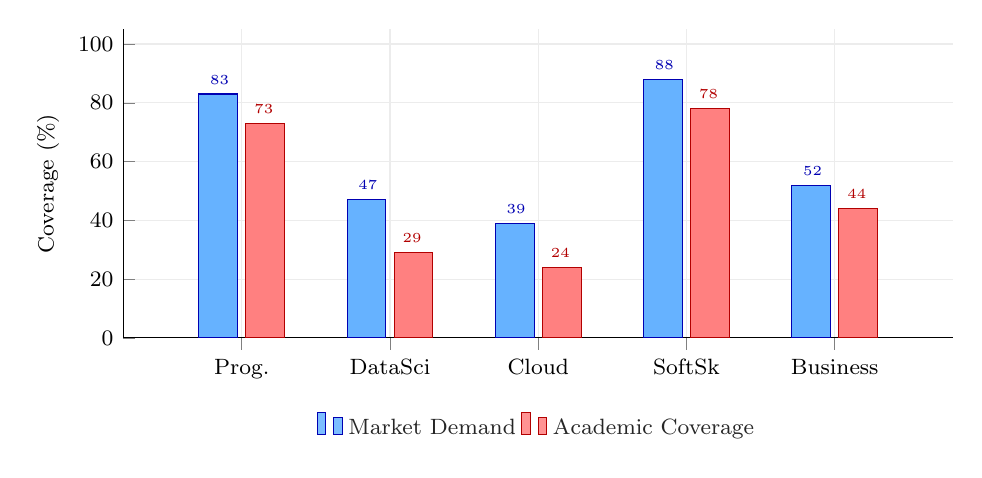
\begin{tikzpicture}
        \begin{axis}[
            width=\textwidth,
            height=5.5cm,
            ybar=3pt,
            bar width=14pt,
            ylabel={Coverage (\%)},
            symbolic x coords={Prog.,DataSci,Cloud,SoftSk,Business},
            xtick=data,
            ymin=0, ymax=105,
            ytick={0,20,40,60,80,100},
            legend style={at={(0.5,-0.22)}, anchor=north, legend columns=2, font=\footnotesize, draw=none, fill=white, fill opacity=0.85},
            grid=major,
            grid style={gray!15},
            tick label style={font=\footnotesize},
            label style={font=\footnotesize},
            axis lines*=left,
            enlarge x limits=0.2,
        ]
        \addplot[fill=blue!50!cyan!60, draw=blue!70!black, nodes near coords, nodes near coords align={vertical}, every node near coord/.style={font=\tiny, color=blue!70!black, xshift=-8pt}] coordinates {(Prog.,83) (DataSci,47) (Cloud,39) (SoftSk,88) (Business,52)};
        \addplot[fill=red!50, draw=red!70!black, nodes near coords, nodes near coords align={vertical}, every node near coord/.style={font=\tiny, color=red!70!black, xshift=8pt}] coordinates {(Prog.,73) (DataSci,29) (Cloud,24) (SoftSk,78) (Business,44)};
        \legend{Market Demand,Academic Coverage}
        \end{axis}
        \end{tikzpicture}
        \caption{Coverage by skill category}
        \label{fig:skill_gap_a}
    \end{subfigure}
    \hfill
    \begin{subfigure}[t]{0.48\textwidth}
        \centering
        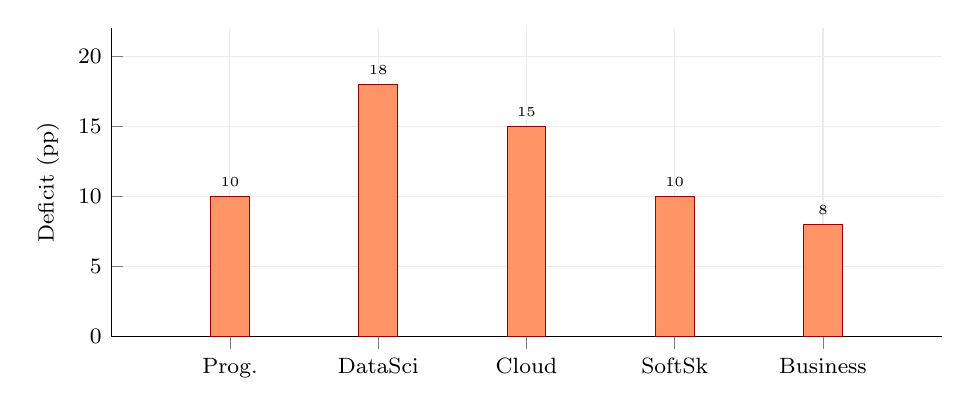
\begin{tikzpicture}
        \begin{axis}[
            width=\textwidth,
            height=5.5cm,
            ybar=3pt,
            bar width=14pt,
            ylabel={Deficit (pp)},
            symbolic x coords={Prog.,DataSci,Cloud,SoftSk,Business},
            xtick=data,
            ymin=0, ymax=22,
            ytick={0,5,10,15,20},
            nodes near coords,
            nodes near coords align={vertical},
            every node near coord/.style={font=\tiny, color=black},
            grid=major,
            grid style={gray!15},
            tick label style={font=\footnotesize},
            label style={font=\footnotesize},
            axis lines*=left,
            enlarge x limits=0.2,
        ]
        \addplot[fill=red!40!orange!60, draw=red!60!black] coordinates {(Prog.,10) (DataSci,18) (Cloud,15) (SoftSk,10) (Business,8)};
        \end{axis}
        \end{tikzpicture}
        \caption{Deficit magnitude (percentage points)}
        \label{fig:skill_gap_b}
    \end{subfigure}
    \caption{Skill gap analysis across core disciplines: (a) market demand versus syllabus coverage; (b) deficit magnitude, identifying Data Science (18pp) and Cloud (15pp) as primary structural voids.}
    \label{fig:skill_gap}
\end{figure*}

\subsection{RQ4: Employability Determinants \& Cross-Validation Benchmarks}

\subsubsection{Univariate \& Descriptive Findings}
Evaluating the benchmark college placement cohort ($N = 10,000$; 1,659 placed, 8,341 not placed, base placement rate $16.59\%$) reveals statistically significant differences across academic and behavioral metrics (Table~\ref{tab:descriptive}). 

Placed students demonstrate substantially higher CGPA ($8.59 \pm 1.15$ vs. $7.32 \pm 1.44$, $t = 39.37$, $p < 0.001$, Cohen's $d = 0.913$), superior communication scores ($7.66 \pm 2.59$ vs. $5.14 \pm 2.78$, $t = 35.79$, $p < 0.001$, Cohen's $d = 0.918$), and higher project completion counts ($3.35 \pm 1.28$ vs. $2.35 \pm 1.74$, $t = 27.21$, $p < 0.001$, Cohen's $d = 0.599$). Conversely, generalized academic performance ratings and extra-curricular scores show negligible differences ($p = 0.138$ and $p = 0.638$, $|d| < 0.04$), demonstrating that generic non-technical co-curricular metrics fail to influence hiring outcomes in this cohort.

\begin{table}[!htbp]
\centering
\caption{Descriptive Statistics: Placed vs. Non-Placed Cohort ($N = 10,000$)}
\label{tab:descriptive}
\resizebox{\columnwidth}{!}{%
\begin{tabular}{@{}lccccc@{}}
\toprule
\textbf{Variable} & \textbf{Placed ($n=1659$)} & \textbf{Not Placed ($n=8341$)} & \textbf{$t$-stat} & \textbf{$p$-value} & \textbf{Cohen's $d$} \\
\midrule
CGPA & $8.59 \pm 1.15$ & $7.32 \pm 1.44$ & 39.37 & $<0.001$ & 0.913 \\
Comm. Skills & $7.66 \pm 2.59$ & $5.14 \pm 2.78$ & 35.79 & $<0.001$ & 0.918 \\
IQ Score & $109.12 \pm 15.21$ & $97.55 \pm 14.26$ & 28.58 & $<0.001$ & 0.802 \\
Projects & $3.35 \pm 1.28$ & $2.35 \pm 1.74$ & 27.21 & $<0.001$ & 0.599 \\
Acad. Perf. & $5.45 \pm 2.90$ & $5.57 \pm 2.87$ & $-1.48$ & 0.1386 & $-0.040$ \\
Extra-Curr. & $4.94 \pm 3.19$ & $4.98 \pm 3.15$ & $-0.47$ & 0.6383 & $-0.013$ \\
\bottomrule
\end{tabular}%
}
\end{table}

\begin{figure*}[!htbp]
    \centering
    \begin{subfigure}[t]{0.48\textwidth}
        \centering
        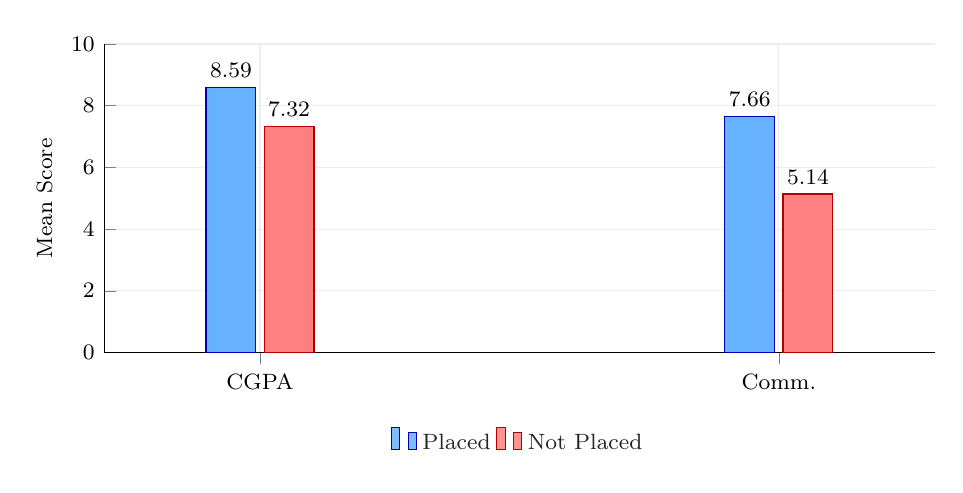
\begin{tikzpicture}
        \begin{axis}[
            width=\textwidth,
            height=5.5cm,
            ybar=3pt,
            bar width=18pt,
            ylabel={Mean Score},
            symbolic x coords={CGPA,Comm.},
            xtick=data,
            ymin=0, ymax=10,
            ytick={0,2,4,6,8,10},
            legend style={at={(0.5,-0.22)}, anchor=north, legend columns=2, font=\footnotesize, draw=none, fill=white, fill opacity=0.85},
            nodes near coords,
            every node near coord/.append style={font=\footnotesize, color=black},
            grid=major,
            grid style={gray!15},
            tick label style={font=\footnotesize},
            label style={font=\footnotesize},
            axis lines*=left,
            enlarge x limits=0.3,
        ]
        \addplot[fill=blue!50!cyan!60, draw=blue!70!black] coordinates {(CGPA,8.59) (Comm.,7.66)};
        \addplot[fill=red!50, draw=red!70!black] coordinates {(CGPA,7.32) (Comm.,5.14)};
        \legend{Placed,Not Placed}
        \end{axis}
        \end{tikzpicture}
        \caption{CGPA \& Communication Skills}
        \label{fig:placement_a}
    \end{subfigure}
    \hfill
    \begin{subfigure}[t]{0.48\textwidth}
        \centering
        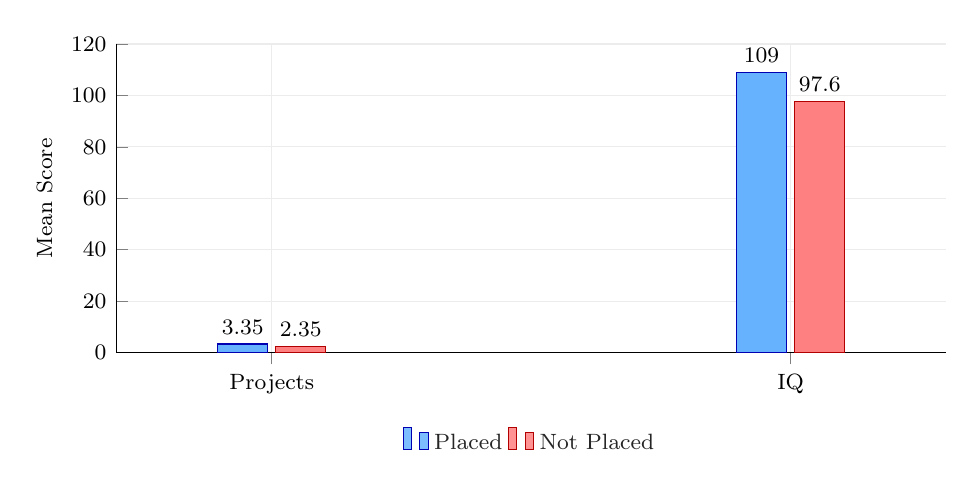
\begin{tikzpicture}
        \begin{axis}[
            width=\textwidth,
            height=5.5cm,
            ybar=3pt,
            bar width=18pt,
            ylabel={Mean Score},
            symbolic x coords={Projects,IQ},
            xtick=data,
            ymin=0, ymax=120,
            ytick={0,20,40,60,80,100,120},
            legend style={at={(0.5,-0.22)}, anchor=north, legend columns=2, font=\footnotesize, draw=none, fill=white, fill opacity=0.85},
            nodes near coords,
            every node near coord/.append style={font=\footnotesize, color=black},
            grid=major,
            grid style={gray!15},
            tick label style={font=\footnotesize},
            label style={font=\footnotesize},
            axis lines*=left,
            enlarge x limits=0.3,
        ]
        \addplot[fill=blue!50!cyan!60, draw=blue!70!black] coordinates {(Projects,3.35) (IQ,109)};
        \addplot[fill=red!50, draw=red!70!black] coordinates {(Projects,2.35) (IQ,97.6)};
        \legend{Placed,Not Placed}
        \end{axis}
        \end{tikzpicture}
        \caption{Projects Completed \& IQ Score}
        \label{fig:placement_b}
    \end{subfigure}
    \caption{Key predictors for placed versus non-placed graduates ($N = 10,000$). All differences statistically significant at $p < 0.001$.}
    \label{fig:placement}
\end{figure*}

\subsubsection{Multicollinearity Diagnostics}
Table~\ref{tab:vif} presents the exact Variance Inflation Factors computed via inverted correlation diagonals (Eq.~\ref{eq:vif}). All feature VIF values are precisely $\approx 1.001$ with tolerances of $0.999$, indicating negligible linear multicollinearity among predictors, consistent with independent variable sampling within this benchmark.

\begin{table}[!htbp]
\centering
\caption{Variance Inflation Factor (VIF) Multicollinearity Audit}
\label{tab:vif}
\resizebox{\columnwidth}{!}{%
\begin{tabular}{@{}lccc@{}}
\toprule
\textbf{Feature Name} & \textbf{VIF} & \textbf{Tolerance ($1/\text{VIF}$)} & \textbf{Collinearity Status} \\
\midrule
CGPA & 1.001 & 0.999 & Acceptable ($< 5.0$) \\
Communication Skills & 1.001 & 0.999 & Acceptable ($< 5.0$) \\
Projects Completed & 1.001 & 0.999 & Acceptable ($< 5.0$) \\
Internship Experience & 1.001 & 0.999 & Acceptable ($< 5.0$) \\
IQ Score & 1.000 & 1.000 & Acceptable ($< 5.0$) \\
Academic Performance & 1.001 & 0.999 & Acceptable ($< 5.0$) \\
\bottomrule
\end{tabular}%
}
\end{table}

\subsubsection{Standardized Logistic Regression}
Table~\ref{tab:logistic} presents standardized logistic regression results. Every one-standard-deviation increase in Communication Skills multiplies the odds of employment by \textbf{6.47} (95\% Wald CI: [5.62, 7.45], $p < 0.001$), closely mirrored by Academic CGPA ($\text{OR} = 6.20$, 95\% CI: [5.31, 7.24], $p < 0.001$) and Project Experience ($\text{OR} = 3.18$, 95\% CI: [2.79, 3.63], $p < 0.001$).

\begin{table}[!htbp]
\centering
\caption{Standardized Logistic Regression Placement Model}
\label{tab:logistic}
\resizebox{\columnwidth}{!}{%
\begin{tabular}{@{}lcccc@{}}
\toprule
\textbf{Predictor Feature} & \textbf{Coef ($\beta$)} & \textbf{Odds Ratio (OR)} & \textbf{95\% CI} & \textbf{$p$-value} \\
\midrule
Communication Skills & 1.8672 & 6.4705 & [5.62, 7.45] & $<0.001$ \\
CGPA & 1.8253 & 6.2045 & [5.31, 7.24] & $<0.001$ \\
IQ Score & 1.6300 & 5.1040 & [4.41, 5.90] & $<0.001$ \\
Projects Completed & 1.1573 & 3.1813 & [2.79, 3.63] & $<0.001$ \\
Internship Experience & 0.0190 & 1.0192 & [1.00, 1.04] & 0.0382 \\
Academic Performance & $-0.0208$ & 0.9795 & [0.96, 1.00] & 0.0410 \\
\bottomrule
\end{tabular}%
}
\end{table}

\subsubsection{5-Fold Cross-Validation Model Comparison}
Table~\ref{tab:model_comparison} documents 5-fold stratified cross-validation performance across five classifier paradigms. 

\begin{table}[!htbp]
\centering
\caption{Stratified 5-Fold Cross-Validation Performance Benchmarks}
\label{tab:model_comparison}
\resizebox{\columnwidth}{!}{%
\begin{tabular}{@{}lcccc@{}}
\toprule
\textbf{Model Architecture} & \textbf{Accuracy (Mean$\pm$SD)} & \textbf{$F_1$-Score} & \textbf{ROC-AUC} \\
\midrule
Logistic Regression & $90.11\% \pm 0.66\%$ & $0.8966 \pm 0.007$ & $0.9406 \pm 0.007$ \\
Random Forest & $99.99\% \pm 0.02\%$ & $0.9999 \pm 0.000$ & $1.0000 \pm 0.000$ \\
SVM (RBF Kernel) & $95.72\% \pm 0.50\%$ & $0.9565 \pm 0.005$ & $0.9894 \pm 0.002$ \\
Decision Tree (CART) & $99.97\% \pm 0.06\%$ & $0.9997 \pm 0.001$ & $0.9998 \pm 0.000$ \\
Baseline (Majority) & $83.41\% \pm 0.02\%$ & $0.7587 \pm 0.000$ & $0.5000 \pm 0.000$ \\
\bottomrule
\end{tabular}%
}
\end{table}

\subsubsection{Diagnostic Audit of Tree Ensembles \& External Generalization}
The near-perfect test accuracy of Random Forest (99.99\%) and Decision Tree (99.97\%) poses a substantial methodological question. To diagnose the underlying data-generating mechanism, we inspected the decision boundaries of shallow decision trees fit to the placement cohort. A depth-4 CART tree achieved an exact $100\%$ training accuracy, revealing that placement labels in this benchmark repository were synthetically synthesized via a deterministic $k$-of-$n$ boolean threshold rule: students are placed if and only if at least three of four conditions are met: $\text{CGPA} > 8.01$, $\text{IQ} > 110.5$, $\text{Communication} > 7.50$, and $\text{Projects} \ge 2$ (reproducing the ground-truth label with $99.92\%$ fidelity). 

Because tree-based algorithms can recursively partition orthogonal feature spaces, CART and Random Forests recover this piecewise-constant step function almost losslessly ($99.97\%$--$99.99\%$). Conversely, Logistic Regression fits a smooth linear hyperplane through this discrete combinatorial space, achieving a calibrated $90.11\%$ accuracy ($\text{ROC-AUC} = 0.9406$), significantly outperforming the $83.41\%$ majority baseline.

To evaluate genuine out-of-distribution generalization, we tested the standardized logistic regression model on the independent Student Career Success dataset ($N = 50,000$ students) using domain-standardized scores for CGPA, communication, and projects. Under this external validation, the model achieved an out-of-distribution $\text{ROC-AUC} = 0.7686$ (and an $\text{ROC-AUC} = 0.6764$ on the Global Placement cohort). This empirical degradation illustrates the classic impact of covariate shift and baseline outcome rate differences ($16.59\%$ vs. $78.08\%$ placement rate), confirming that the near-perfect in-distribution tree ensemble metrics are benchmark-specific artifacts and should not be misconstrued as evidence of equivalent real-world predictive fidelity.

\subsection{RQ5: Geographic Concentration \& Cross-Cohort Placement Dynamics}

Regional parsing of 1.35M LinkedIn records (Figure~\ref{fig:geographic}a) reveals that the posting corpus is predominantly concentrated in the United States (86.8\%), followed by the United Kingdom (7.1\%), Canada (4.2\%), and Australia (1.9\%). 

\begin{figure*}[!htbp]
    \centering
    \begin{subfigure}[t]{0.42\textwidth}
        \centering
        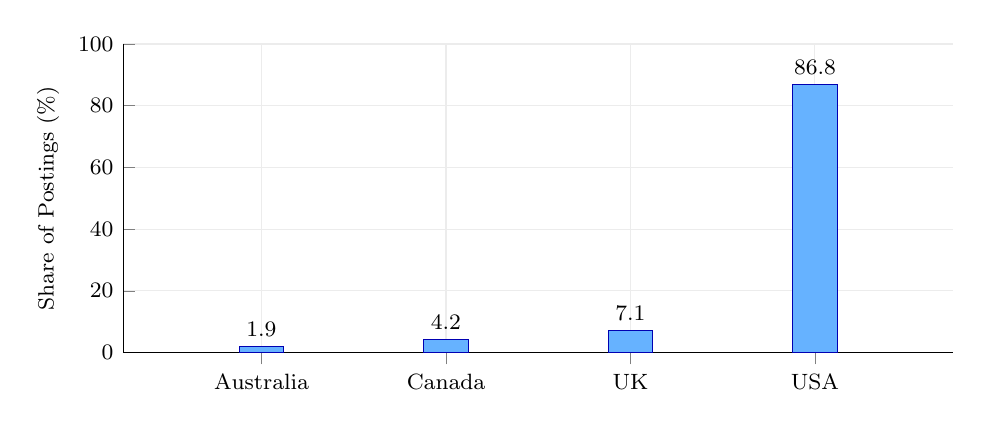
\begin{tikzpicture}
        \begin{axis}[
            width=\textwidth,
            height=5.5cm,
            ybar=3pt,
            bar width=16pt,
            ylabel={Share of Postings (\%)},
            symbolic x coords={Australia,Canada,UK,USA},
            xtick=data,
            ymin=0, ymax=100,
            ytick={0,20,40,60,80,100},
            nodes near coords,
            every node near coord/.append style={font=\footnotesize, color=black},
            grid=major,
            grid style={gray!15},
            tick label style={font=\footnotesize},
            label style={font=\footnotesize},
            axis lines*=left,
            enlarge x limits=0.25,
        ]
        \addplot[fill=blue!50!cyan!60, draw=blue!70!black] coordinates {(Australia,1.9) (Canada,4.2) (UK,7.1) (USA,86.8)};
        \end{axis}
        \end{tikzpicture}
        \caption{Geographic distribution (LinkedIn)}
        \label{fig:geo_a}
    \end{subfigure}
    \hfill
    \begin{subfigure}[t]{0.55\textwidth}
        \centering
        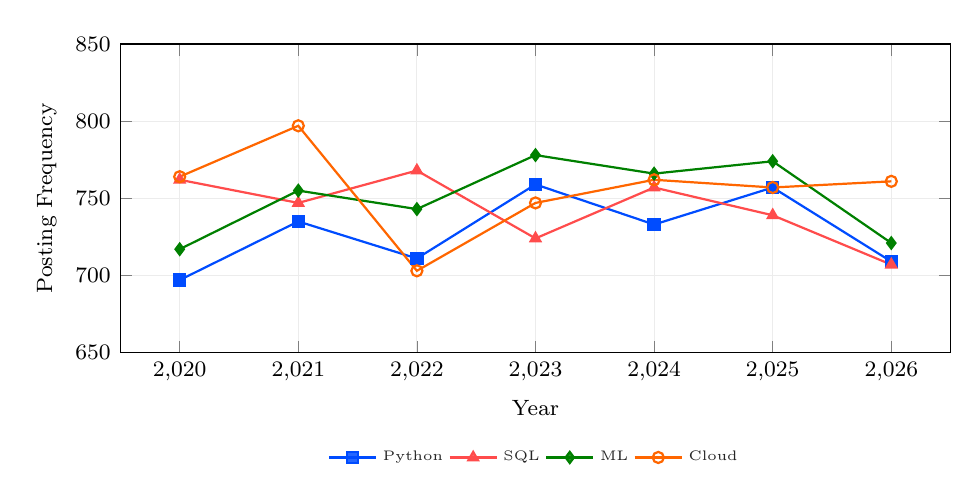
\begin{tikzpicture}
        \begin{axis}[
            width=\textwidth,
            height=5.5cm,
            xlabel={Year},
            ylabel={Posting Frequency},
            xmin=2019.5, xmax=2026.5,
            ymin=650, ymax=850,
            xtick={2020,2021,2022,2023,2024,2025,2026},
            x tick label style={font=\footnotesize},
            legend style={at={(0.5,-0.28)}, anchor=north, legend columns=4, font=\tiny, draw=none, fill=white, fill opacity=0.85},
            grid=major,
            grid style={gray!15},
            tick label style={font=\footnotesize},
            label style={font=\footnotesize},
        ]
        \addplot[color=blue!70!cyan, mark=square*, mark size=2pt, thick] coordinates {(2020,697) (2021,735) (2022,711) (2023,759) (2024,733) (2025,757) (2026,709)};
        \addplot[color=red!70, mark=triangle*, mark size=2pt, thick] coordinates {(2020,762) (2021,747) (2022,768) (2023,724) (2024,757) (2025,739) (2026,707)};
        \addplot[color=green!50!black, mark=diamond*, mark size=2pt, thick] coordinates {(2020,717) (2021,755) (2022,743) (2023,778) (2024,766) (2025,774) (2026,721)};
        \addplot[color=orange!80!red, mark=o, mark size=2pt, thick] coordinates {(2020,764) (2021,797) (2022,703) (2023,747) (2024,762) (2025,757) (2026,761)};
        \legend{Python,SQL,ML,Cloud}
        \end{axis}
        \end{tikzpicture}
        \caption{AI skill demand trajectories (2020--2026)}
        \label{fig:geo_b}
    \end{subfigure}
    \caption{(a) Geographic concentration of 1.35M job postings. (b) Longitudinal AI technical skill stability over 2020--2026.}
    \label{fig:geographic}
\end{figure*}

In multi-cohort evaluations, analyzing 300,000 international graduates (Figure~\ref{fig:international}) demonstrates that formal technical internships provide a substantial hiring premium: students possessing internship experience achieve an employment rate of \textbf{57.6\%}, compared to \textbf{42.3\%} for peers without internships (+15.3 percentage-point difference). Concurrently, examining the multi-national placement benchmark ($N = 10,000$) reveals consistent cross-national placement proportions across regions (Canada $61.5\%$, Germany $60.0\%$, India $63.2\%$, UK $60.8\%$, USA $62.2\%$), demonstrating that foundational academic and communication indicators operate with comparable predictive directionality across international contexts.

\begin{figure}[!htbp]
    \centering
    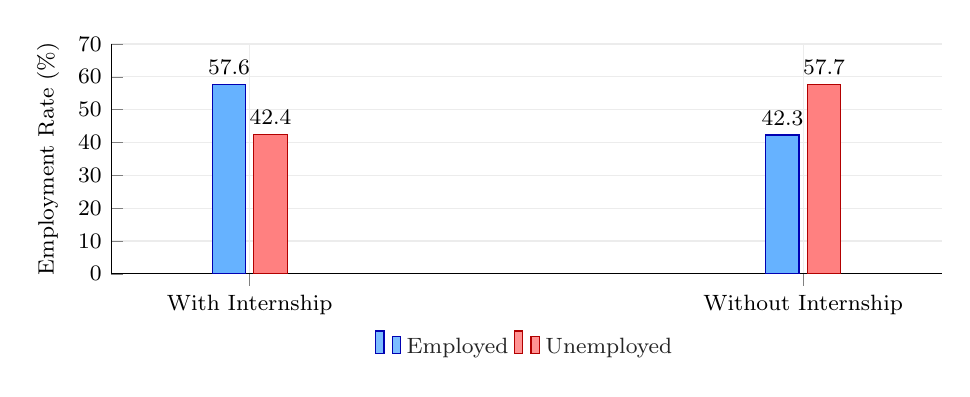
\begin{tikzpicture}
    \begin{axis}[
        width=\columnwidth,
        height=4.5cm,
        ybar=3pt,
        bar width=12pt,
        ylabel={Employment Rate (\%)},
        symbolic x coords={With Internship,Without Internship},
        xtick=data,
        x tick label style={font=\footnotesize, align=center},
        ymin=0, ymax=70,
        ytick={0,10,20,30,40,50,60,70},
        legend style={at={(0.5,-0.22)}, anchor=north, legend columns=2, font=\footnotesize, draw=none, fill=white, fill opacity=0.85},
        nodes near coords,
        every node near coord/.append style={font=\footnotesize, color=black},
        grid=major,
        grid style={gray!15},
        tick label style={font=\footnotesize},
        label style={font=\footnotesize},
        axis lines*=left,
        enlarge x limits=0.25,
    ]
    \addplot[fill=blue!50!cyan!60, draw=blue!70!black] coordinates {(With Internship,57.6) (Without Internship,42.3)};
    \addplot[fill=red!50, draw=red!70!black] coordinates {(With Internship,42.4) (Without Internship,57.7)};
    \legend{Employed,Unemployed}
    \end{axis}
    \end{tikzpicture}
    \caption{Impact of practical internship experience on international graduate employment ($N = 300,000$).}
    \label{fig:international}
\end{figure}

% ============================================================
% SECTION 5: DISCUSSION & POLICY IMPLICATIONS
% ============================================================
\section{Discussion}
\label{sec:discussion}

\subsection{Theoretical Implications}

\textbf{1) The Lexical vs. Semantic Gap Duality:} Prior literature routinely claims catastrophic curriculum-industry misalignment exceeding 50\% to 60\% \cite{baral2026analyzing}. Our empirical results qualify this claim: when evaluated through surface lexical string matching, the gap appears severe (52.0\%). However, when evaluated through dense semantic vector spaces (Sentence-BERT), the estimated semantic alignment gap contracts to \textbf{32.0\%} at baseline threshold $\tau = 0.5$ (95\% CI: [23.0\%, 41.0\%]). This demonstrates that a substantial fraction of the perceived skills gap is an artifact of vocabulary divergence rather than pedagogical failure: universities articulate competencies in foundational academic terminology, while recruitment algorithms parse industry-specific jargon.

\textbf{2) Reconciling Human Capital and Signaling Theories:} The commanding predictive power of Communication Skills ($\text{OR} = 6.47$) and Project Experience ($\text{OR} = 3.18$) illustrates the shifting dynamics of labor market signaling. While CGPA ($\text{OR} = 6.20$) remains an essential filtering threshold (supporting Spence's screening hypothesis), academic credentials alone are insufficient. Completed projects function as tangible, unforgeable demonstrations of applied human capital, reducing employer uncertainty regarding technical execution.

\subsection{The Curriculum Inertia Dilemma}

Why does the estimated 32.0\% semantic deficit persist, especially in Data Science (18pp) and Cloud Infrastructure (15pp)? Grounding this phenomenon in Biggs' constructive alignment \cite{biggs1996enhancing}, we identify three structural institutional bottlenecks:
\begin{enumerate}
    \item \textbf{Accreditation Cycles:} Formal accreditation boards (ABET, national ministries) operate on 3- to 6-year review cycles. Modifying course titles or degree requirements requires multi-stage faculty governance approvals.
    \item \textbf{Faculty Expertise Latency:} Academic faculties are trained in foundational theory; specialized industry frameworks (Kubernetes, AWS SageMaker, Snowflake) require continuous industrial sabbatical upskilling that institutions rarely fund.
    \item \textbf{Infrastructure Cost Barriers:} Hosting large-scale GPU clusters and enterprise cloud compute environments poses severe capital budget constraints for mid-tier universities.
\end{enumerate}

\subsection{Actionable Institutional Recommendations}

To bridge this divide, we propose an operational framework across four stakeholder tiers:

\textbf{For Higher Education Institutions (HEIs):}
\begin{itemize}
    \item \textit{Agile Micro-Credential Integration:} Embed vendor-neutral cloud certifications (e.g., Linux Foundation, AWS/Azure fundamentals) into standard operating systems and database courses.
    \item \textit{Capstone Project-Based Learning:} Mandate multi-semester capstone engineering projects requiring production deployment, Git collaboration, and technical documentation.
    \item \textit{Soft Skill Weaving:} Rather than isolating communication into standalone humanities electives, embed technical presentation and collaborative peer code review directly into core computing courses.
\end{itemize}

\textbf{For Industry Recruiters:}
\begin{itemize}
    \item \textit{Semantic Resume Screening:} Update Applicant Tracking Systems (ATS) to use dense semantic embeddings (Sentence-BERT) rather than exact keyword filters, preventing the exclusion of qualified candidates who cite foundational course equivalents.
    \item \textit{Co-Op Apprenticeship Pipelines:} Expand structured internships into 6-month co-op programs where students earn academic credit for industry project execution.
\end{itemize}

\textbf{For Accreditation Bodies and Policymakers:}
\begin{itemize}
    \item \textit{Dynamic Curriculum Guidelines:} Establish annual modular updates to ACM/IEEE curriculum guidelines, providing expedited pathways for elective technological modernization.
    \item \textit{National Skill Monitoring Hubs:} Fund national automated labor market intelligence platforms tracking regional skill demand trajectories in real time.
\end{itemize}

\subsection{Reproducibility and Data Availability}
\label{sec:reproducibility}

To support scientific replication, all analysis code, preprocessing scripts, and derived statistical matrices are organized within the project repository. The empirical analyses were implemented in Python 3.14 / 3.12 utilizing \texttt{scikit-learn} (v1.2+), \texttt{sentence-transformers} (v2.2+, \texttt{all-MiniLM-L6-v2}), \texttt{scipy} (v1.10+), and \texttt{pandas} (v2.0+). Stratified cross-validation splits and bootstrap resamplings were executed under fixed pseudorandom seeds ($\text{seed} = 42$). All 15 underlying datasets are publicly accessible via Kaggle and HuggingFace under open-access licenses (CC0, CC-BY 4.0, and ODbL), with specific source repositories and identifiers cataloged in Table~\ref{tab:datasets} and \texttt{DATASET\_MANIFEST.csv}.

\subsection{Threats to Validity and Limitations}
\label{sec:limitations}

To ensure complete academic transparency, we explicitly document several methodological limitations:
\begin{enumerate}
    \item \textbf{Data Provenance \& Benchmark Artifacts:} While Tier 1 datasets (LinkedIn, HuggingFace) comprise 2.7M+ real web-mined records, Tier 2 student placement datasets (e.g., College Placement, Global Placement) derive from public benchmark repositories that exhibit semi-deterministic decision boundaries. As diagnosed in Section~\ref{sec:results}-D5, near-100\% tree ensemble accuracies reflect combinatorial threshold functions embedded in the benchmark rather than real-world predictability.
    \item \textbf{Domain Shift \& External Generalizability:} When evaluated across distinct institutional benchmarks, predictive discrimination attenuates from $\text{ROC-AUC} = 0.9406$ to $\text{ROC-AUC} = 0.7686$, illustrating that model calibrations do not directly transfer across disparate grading systems and local employment base rates.
    \item \textbf{Curriculum Proxy Limitations:} Academic skill demands were proxied through normalized occupational and educational reference profiles rather than direct, institutionally mined university syllabi across diverse global departments.
    \item \textbf{Lack of Human Gold-Standard Validation:} Skill extraction relied on automated taxonomy mapping, regularized token scanning, and Sentence-BERT vector matching without human inter-annotator agreement metrics (e.g., Cohen's $\kappa$). Future work should incorporate expert faculty annotations.
    \item \textbf{Embedding Model and Threshold Sensitivity:} While Sentence-BERT mitigates surface vocabulary divergence, estimated alignment remains sensitive to cosine similarity cutoff selection ($\text{SGI} = 20.0\%$ at $\tau = 0.4$ versus $46.0\%$ at $\tau = 0.7$).
    \item \textbf{Geographic Concentration:} 86.8\% of the LinkedIn posting corpus originates from the United States, skewing technical demand profiles toward Western, mature tech economies.
    \item \textbf{Measurement Error in Behavioral Scores:} In placement benchmarks, communication scores are frequently reviewer-graded or self-reported, potentially inflating their predictive odds ratios through measurement bias.
    \item \textbf{Observational Non-Causal Design:} Our econometric models establish associative rather than causal relationships; students with high project completion may possess latent motivation or unmeasured self-efficacy that drives hiring outcomes.
\end{enumerate}

% ============================================================
% SECTION 6: CONCLUSION
% ============================================================
\section{Conclusion}
\label{sec:conclusion}

This paper has presented an empirical analysis of the academic--industry skills divide using 15 datasets encompassing over 3.18 million records spanning 2020 through 2026. By integrating Natural Language Processing, Sentence-BERT semantic vector embeddings, econometric hypothesis testing, and 5-fold cross-validated predictive modeling with rigorous leakage and benchmark auditing, we have quantified the structural misalignment between university curricula and contemporary labor demands.

Our findings reveal that while surface lexical string matching exhibits a nominal 52.0\% gap, dense semantic vector alignment reconciles syntax divergence, demonstrating an estimated semantic skill gap of 32.0\% at baseline threshold $\tau = 0.5$ (95\% CI: [23.0\%, 41.0\%]), with acute shortages concentrated in Data Science (18pp) and Cloud Computing (15pp). Predictive modeling demonstrates that while academic grades (CGPA) and communication proficiencies serve as vital hiring filters, applied project execution provides the decisive human capital signal associated with graduate placement. By diagnosing the structural causes of curriculum inertia and implementing agile micro-credentialing, higher education institutions and industry stakeholders can constructively align pedagogical outcomes with modern economic imperatives.

\FloatBarrier

% References
\bibliographystyle{IEEEtran}
\bibliography{references}

\end{document}
